\chapter{Konzeption des Generative Adversarial Networks}
\label{chap:konzept}
\section{Datensatz}
Analog zu der in Kapitel \ref{chap:vorherige-arbeiten-rub} beschriebenen Arbeit wird der \ac{GTSRB} als Datensatz für diese Studienarbeit verwendet. Dies hängt mit der Größe des Datensatzes zusammen, mit der vergleichsweise kleinen Auflösung der einzelnen Bilder und damit, dass sich diese Arbeit auf die Genereriung deutscher Straßenschilder beschränkt. Es soll jedoch in Kapitel \ref{chap:Evaluation} ebenfalls geprüft werden, inwiefern das Resultat der Arbeit genutzt werden kann, um Bilder zu generieren, die Straßenschilder aus anderen Ländern zeigen. Länder, die das Wiener Übereinkommen über Straßenschilder unterzeichnet haben, besitzen vergleichsweise ähnlich aussehende Straßenschilder. Durch das Übereinkommen wird mitunter die grundlegende Form und Farbe verschiedener Schilder bestimmt. \cite{vienna-convention} \cite{GTSRB}

Der \ac{GTSRB} besteht aus mehr als 50.000 Bildern verteilt auf 43 Klassen respektive 43 verschiedenen Arten von Straßenschildern. Beispiele aus dem Datensatz sind in folgender Abbildung dargestellt.
\begin{figure}[H]
   \centering
   \begin{subfigure}[b]{0.125\textwidth}
       \centering
       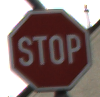
\includegraphics[height=\textwidth]{../images/GTSRB/00093.png}
       \caption{}
       \label{fig:gtrsb-paper-bsp-image-1}
   \end{subfigure}
   \hspace{3em}%
   \begin{subfigure}[b]{0.125\textwidth}
       \centering
       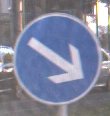
\includegraphics[height=\textwidth]{../images/GTSRB/00847.png}
       \caption{}
       \label{fig:gtrsb-paper-bsp-image-2}
   \end{subfigure}
   \hspace{3em}%
   \begin{subfigure}[b]{0.125\textwidth}
       \centering
       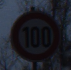
\includegraphics[height=\textwidth]{../images/GTSRB/00040.png}
       \caption{}
       \label{fig:gtrsb-paper-bsp-image-3}
   \end{subfigure}
   \hspace{3em}%
   \begin{subfigure}[b]{0.125\textwidth}
    \centering
    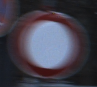
\includegraphics[height=\textwidth]{../images/GTSRB/00052.png}
    \caption{}
    \label{fig:gtrsb-paper-bsp-image-4}
\end{subfigure}
      \caption{Beispielbilder aus dem \acs{GTSRB} Datensatz \cite{GTSRB}}
      \label{fig:gtrsb-paper-bsp-images}
\end{figure}

Die Bilder des Datensatzes besitzen unterschiedliche Seitenverhältnisse und verschiedene Auflösungen. Ein Großteil der Bilder ist jedoch kleiner als 100x100 Pixel. Die Bilder basieren auf Videos, die durch die Autoren tagsüber im Straßenverkehr aufgenommen wurden. Die Trainingsbilder sind ungleich auf die Anzahl an Klassen verteilt. Dies hängt mitunter damit zusammen, dass die jeweiligen Schilder nicht gleich häufig im Straßenverkehr verwendet werden. Unterteilt wird der Datensatz in 39.209 Trainingsbilder und 12.630 Testbilder. Da das Ziel dieser Arbeit jedoch nicht ist, einen Klassifikator mit den generierten Bildern zu trainieren, können auch die Testbilder für das Training des Netzes verwendet werden. Es wird nicht zwischen Trainings- und Testbildern unterschieden. \cite{GTSRB}

Der Datensatz wird in dieser Arbeit zunächst so präpariert, dass nur Bilder für das Training verwendet werden, die mindestens 50 Pixel breit oder hoch sind. Dies wird im Verlauf geändert, sodass die Mindestgröße 75 Pixel beträgt.
\section{Framework}
\section{Architektur}
In Kapitel \ref{chap:NoGANs} werden verschiedene generative Netzwerkarchitekturen vorgestellt. Zunächst soll darauf eingegangen werden, welche dieser Herangehensweisen gewählt wird. Jede der Architekturen besitzt ihre Vor- und Nachteile. Der größte Nachteil von \acp{PixelRNN} ist, dass die Pixel eines Bildes nicht parallel zueinander generiert werden können. Dies verlangsamt die Generierung und damit das Training des Modells.

\textbf{Entscheidungsmatrix?}

\section{Datenaugmentation}


\section{Training}